
\chapter{Übersicht: Beispiel}

\noindent
\begin{center}
	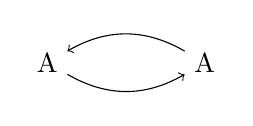
\begin{tikzpicture}
		\node (A) at (-1,0) {A};
		\node (B) at (+1,0) {A};
		\draw [->] (A) to [bend right] (B);
		\draw [->] (B) to [bend right] (A);
	\end{tikzpicture}
	\captionof*{figure}{Diagram}
\end{center}
